\documentclass[11pt,a4paper]{article}
\usepackage[margin=2.5cm]{geometry}
\usepackage[T1]{fontenc}
\usepackage[utf8]{inputenc}
\usepackage{lmodern}
\usepackage{microtype}
\usepackage{booktabs}
\usepackage{graphicx}
\usepackage{amsmath}
\usepackage[round]{natbib}
\usepackage[hidelinks]{hyperref}
\usepackage{xcolor}

\title{Is It the Model or the Labels?\\[2pt]
\large Cross-Lingual Gaps in Hate Speech Detection for English, Hindi and Code-Mixed Hinglish}
\author{Aaditya Kaushik\\
Dhirubhai Ambani University (formerly DA-IICT), Gandhinagar, India\\
\texttt{202401001@dau.ac.in}}
\date{October 2026}

\begin{document}
\maketitle

\begin{center}
\fbox{\parbox{0.9\linewidth}{\small\textbf{Content warning:} this paper discusses hate speech and abusive language. No offensive examples are reproduced in the text.}}
\end{center}

\begin{abstract}
Hate speech classifiers for Indian social media usually perform worse on Hindi and code-mixed Hinglish than on English. This gap is usually blamed on the models.
We test that assumption on PRISM, a public dataset of 29.5K English, Hindi (Devanagari) and Hinglish posts that merges several older corpora.
We compare a TF-IDF baseline, two fine-tuned multilingual transformers (XLM-R and MuRIL) and a zero-shot large language model.
All trained models show a statistically clear 13--20 point macro-F1 gap between English and the Hindi/Hinglish subsets, and moving to stronger or India-specific models does not close it.
We then trace the labels back to their sources.
Each language subset comes from a different original corpus.
For 19\% of the Hindi test posts we can match the original CONSTRAINT-2021 annotation, and on these posts PRISM's labels show no agreement with the original labels beyond chance (Cohen's $\kappa \approx 0$).
On these posts the fine-tuned transformers score below chance (macro-F1 $\approx 0.40$). On the remaining Hindi posts they score 0.64--0.66.
Removing the matched posts from training barely changes results, so the damage is mainly to evaluation.
Cross-model agreement, a manual re-annotation of model errors and a blind re-annotation of random posts point the same way.
We conclude that a substantial part of the measured cross-lingual gap reflects label quality in the merged dataset rather than model limitations. Language-level comparisons on merged corpora should therefore be preceded by an audit of where the labels come from.
\end{abstract}

\section{Introduction}

India has hundreds of millions of social media users who write in Hindi, English, and \emph{Hinglish}: Hindi written in Latin script and freely mixed with English within a sentence.
Hinglish is hard for NLP systems because it has no standard spelling, it switches language mid-sentence, and most pre-trained models saw relatively little romanised Hindi.
Shared tasks such as HASOC \citep{mandl2019hasoc,mandl2020hasoc,modha2021hasoc} have made hate and offensive content detection in Indo-European languages, including code-mixed Hindi--English, a standard benchmark problem.

A common observation is that classifiers perform worse on Hindi and Hinglish than on English.
The usual explanation is the \emph{model}: tokenisers fragment romanised words, and pre-training data under-represents these languages.
A second, less often tested explanation is the \emph{data}.
If the Hindi and Hinglish labels are noisier, or follow a different definition of hate, then no model can reach English-level scores on them.
This risk is especially high for datasets built by merging older corpora, which is now common for low-resource languages.

This paper asks: \textbf{how much of the English vs.\ Hindi/Hinglish performance gap in hate speech detection is due to the models, and how much is due to the labels?}
Our contributions are:
\begin{enumerate}
  \item A controlled comparison of a classical baseline, two fine-tuned multilingual transformers and a zero-shot LLM, scored per language with bootstrap confidence intervals (Section~\ref{sec:results}).
  \item A provenance audit of a public merged dataset. For a matched subset of Hindi posts, the merged labels are unrelated to the original annotation, and this subset alone accounts for a large part of the Hindi deficit (Section~\ref{sec:provenance}).
  \item Supporting evidence from cross-model agreement, a label-independent zero-shot annotator, and manual and blind re-annotation (Section~\ref{sec:labels}).
\end{enumerate}
All code, predictions and annotations are released.\footnote{\url{https://github.com/AadityaKaushik} (repository link to be added).}

\section{Related Work}

\paragraph{Hate speech in Hindi and Hinglish.}
\citet{bohra2018dataset} released one of the first Hindi--English code-mixed hate speech datasets (4,575 tweets).
\citet{mathur2018detecting} studied offensive tweets in code-switched Hindi--English.
The HASOC shared tasks \citep{mandl2019hasoc,mandl2020hasoc,modha2021hasoc} provide larger multilingual benchmarks with separate hate, offensive and profane classes, and use macro-F1 as the official metric.
The CONSTRAINT 2021 Hindi hostility dataset \citep{bhardwaj2020hostility,patwa2021constraint} labels posts as non-hostile or with one or more of fake, hate, offensive and defamation.

\paragraph{Multilingual pre-trained models.}
XLM-R \citep{conneau2020xlmr} is pre-trained on CommonCrawl text in 100 languages.
MuRIL \citep{khanuja2021muril} is pre-trained on 17 Indian languages and, importantly for Hinglish, also on transliterated text.
Both follow the BERT recipe of masked-language-model pre-training followed by task fine-tuning \citep{devlin2019bert}.

\paragraph{Annotation quality in hate speech.}
Hate speech annotation is known to have low inter-annotator agreement \citep{ross2016measuring}, to be confused with general offensive language \citep{davidson2017automated}, and to carry annotator bias \citep{sap2019risk}.
More broadly, \citet{northcutt2021pervasive} show that label errors in test sets can change model rankings.
LLMs have recently been used as annotators \citep{gilardi2023chatgpt}; we use one only as an independent second opinion on the gold labels, not as a replacement for them.

\section{Data}

We use the PRISM code-mixed hate speech dataset \citep{prism}, a public (MIT-licensed) collection of 29,506 posts with binary labels (1 = hate, 0 = not hate).
Every post is tagged with its language: English, Hindi (Devanagari script) or Hinglish (romanised, code-mixed).
We use the released stratified splits without modification (Table~\ref{tab:data}).
Posts are short (median 18 whitespace tokens).
We chose PRISM over the HASOC data because it is openly available and carries a per-post language tag. Section~\ref{sec:provenance} shows that its merged construction is itself an important factor.

\begin{table}[h]
\centering
\small
\begin{tabular}{lrrrr}
\toprule
Split & English & Hindi & Hinglish & Total \\
\midrule
Train & 8,963 & 5,860 & 2,881 & 17,704 \\
Validation & 1,486 & 978 & 486 & 2,950 \\
Test & 4,545 & 2,900 & 1,407 & 8,852 \\
\midrule
Hate share (test) & 49\% & 45\% & 40\% & 46\% \\
\bottomrule
\end{tabular}
\caption{PRISM splits by language.}
\label{tab:data}
\end{table}

\section{Models}

\paragraph{TF-IDF + logistic regression.}
Posts are represented by TF-IDF weights over word 1--2-grams and character 2--5-grams (word-boundary aware, sublinear TF, minimum document frequency 2).
Character n-grams partly capture spelling variants in romanised Hindi.
The regularisation strength $C \in \{0.5,1,2,4,8\}$ is selected on validation macro-F1 ($C=1$).

\paragraph{Fine-tuned transformers.}
We fine-tune \texttt{xlm-roberta-base} (XLM-R) and \texttt{google/muril-base-cased} (MuRIL) with a linear classification head.
Both use identical settings: maximum length 128 tokens, learning rate $2\times10^{-5}$, batch size 32, 3 epochs, weight decay 0.01, mixed precision, seed 42.
Training uses the Hugging Face \texttt{Trainer} \citep{wolf2020transformers} on a single T4 GPU.
Validation macro-F1 is monitored per epoch; the test set is used once.

\paragraph{Zero-shot LLM.}
To get a judgement that does not depend on the training labels, we prompt Claude Opus 5.5 (\texttt{claude-opus-5-5}) with a short annotation instruction.
The instruction labels a post as hate if it attacks, insults, threatens or demeans a person or group, or uses abusive language against someone, and as not hate if it merely discusses or reports on hateful events.
The model received only post IDs and texts; gold labels were withheld.
Because of cost, it labels a fixed random sample of 300 test posts (100 per language, seed 42).
We originally planned to use Gemini through its API, but the free tier repeatedly failed with rate-limit errors, so the sample was labelled by Claude in a fresh agent session using the same prompt.
Labels were not altered after scoring.

\paragraph{Evaluation.}
We report macro-F1, the unweighted mean of per-class F1, following HASOC.
95\% confidence intervals come from 1,000 bootstrap resamples of the test posts within each language. Model differences use paired resampling.

\section{Results}
\label{sec:results}

\begin{table}[h]
\centering
\small
\begin{tabular}{lccccc}
\toprule
Model & English & Hindi & Hinglish & Gap En$-$Hi & Gap En$-$Hgl \\
\midrule
TF-IDF + LR & .777 {\scriptsize[.765,.789]} & .629 {\scriptsize[.612,.647]} & .623 {\scriptsize[.596,.649]} & .148 {\scriptsize[.127,.169]} & .154 {\scriptsize[.124,.184]} \\
XLM-R & .816 {\scriptsize[.804,.827]} & .615 {\scriptsize[.598,.633]} & .666 {\scriptsize[.642,.690]} & .201 {\scriptsize[.180,.221]} & .150 {\scriptsize[.121,.176]} \\
MuRIL & .802 {\scriptsize[.790,.812]} & .628 {\scriptsize[.611,.646]} & .669 {\scriptsize[.644,.693]} & .173 {\scriptsize[.153,.196]} & .132 {\scriptsize[.104,.162]} \\
\bottomrule
\end{tabular}
\caption{Macro-F1 on the full test set (8,852 posts) with 95\% bootstrap confidence intervals. Overall macro-F1: TF-IDF 0.711, XLM-R 0.731, MuRIL 0.731.}
\label{tab:main}
\end{table}

\begin{figure}[h]
\centering
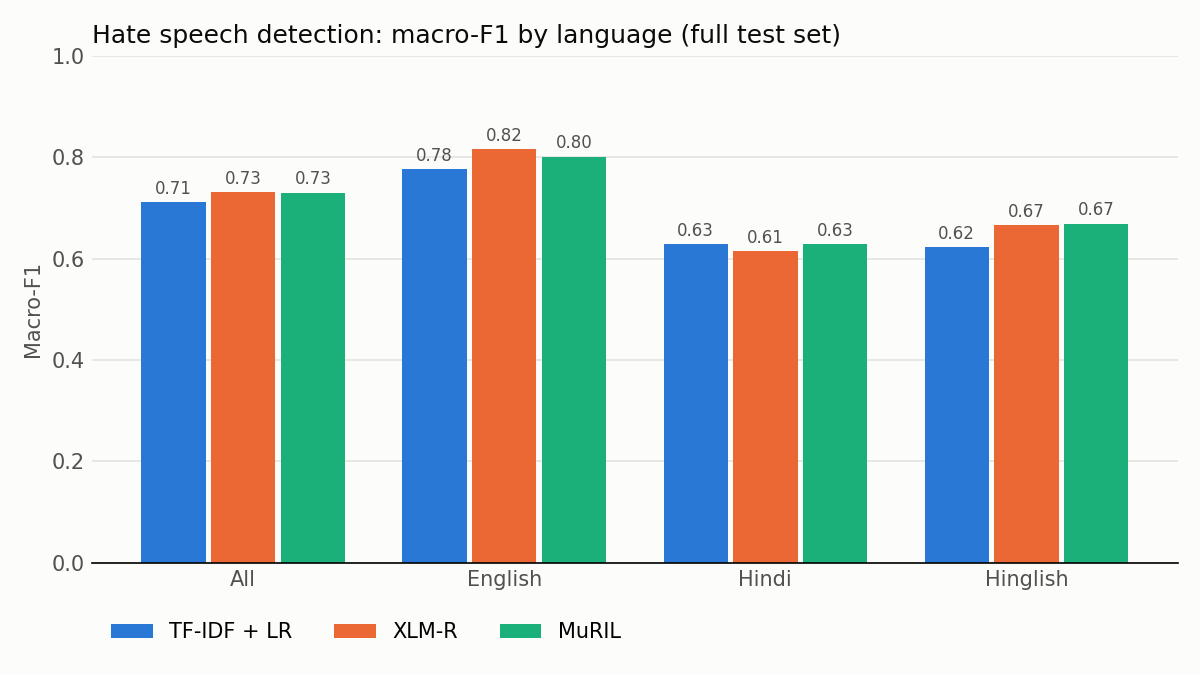
\includegraphics[width=0.85\linewidth]{f1_by_language.png}
\caption{Macro-F1 by language on the full test set.}
\label{fig:main}
\end{figure}

Table~\ref{tab:main} and Figure~\ref{fig:main} show four patterns.

\paragraph{A persistent language gap.}
Every model scores 0.78--0.82 on English but only 0.62--0.67 on Hindi and Hinglish.
All gaps are clearly larger than zero (every confidence interval lies above 0.10).
Moving from a bag-of-n-grams model to multilingual transformers with over 200M parameters raises overall macro-F1 by only two points.

\paragraph{No gain on Devanagari Hindi.}
Compared with TF-IDF, the transformers gain 2.5--4 points on English and about 4.5 points on Hinglish, but nothing on Hindi (0.615--0.628 vs.\ 0.629).
It is surprising that pre-trained multilingual models give no benefit at all on a high-resource script. Section~\ref{sec:provenance} offers an explanation.

\paragraph{MuRIL and XLM-R are close.}
Both reach 0.731 overall.
Paired bootstrap differences (MuRIL $-$ XLM-R) are $-0.014$ [$-0.026$, $-0.003$] on English, $+0.013$ [$0.001$, $0.026$] on Hindi and $+0.004$ [$-0.018$, $0.024$] on Hinglish.
So XLM-R is marginally better on English and MuRIL marginally better on Hindi, while on Hinglish, the case MuRIL's transliteration-aware pre-training targets, we find no difference.
These intervals do not account for training-seed variance, so the small English and Hindi differences should be treated with caution.

\paragraph{Half of Hindi and Hinglish hate is missed.}
Recall on the hate class is 0.75--0.81 for English but only 0.46--0.50 for Hindi and Hinglish for both transformers.

\section{Where Do the Labels Come From?}
\label{sec:provenance}

PRISM's full export includes a \texttt{source} field.
It shows that each language comes from a separate original corpus (Table~\ref{tab:sources}).
All English posts come from one source, sampled to an exact 50/50 class balance.
The main Hinglish source has 4,574 posts with 1,660 hate and 2,914 non-hate, which matches the published statistics of the \citet{bohra2018dataset} dataset (4,575 tweets; 1,661 / 2,914).
A further 209 Hinglish ``posts'' are entries from a profanity word list, all labelled hate. Sixty of them, all single words, are in the Hinglish test set, where they make the Hinglish task look slightly easier than it is.

\begin{table}[h]
\centering
\small
\begin{tabular}{llrr}
\toprule
Language & Source tag in PRISM & Not hate & Hate \\
\midrule
English & \texttt{english\_dataset} & 7,500 & 7,500 \\
Hindi & \texttt{hindi\_dataset} & 5,411 & 4,356 \\
Hinglish & \texttt{hate\_speech\_tsv} & 2,914 & 1,660 \\
Hinglish & \texttt{profanity\_list} & 0 & 209 \\
\bottomrule
\end{tabular}
\caption{Original sources of PRISM posts (full export, before de-duplication).}
\label{tab:sources}
\end{table}

\paragraph{Matching Hindi posts to their original annotation.}
Many PRISM Hindi posts also appear in the CONSTRAINT 2021 Hindi hostility dataset \citep{bhardwaj2020hostility,patwa2021constraint}.
The two datasets clean text differently, so we match posts on the first 60 alphanumeric characters after removing URLs and user mentions, and drop ambiguous keys.
Manual inspection of matched pairs confirms that they are the same posts.
We match 557 of the 2,900 Hindi test posts (19\%).
If PRISM's binary label were derived from the original annotation, it should agree strongly with either CONSTRAINT's \emph{hostile} label or its \emph{hate-or-offensive} label.
Instead, agreement is at chance level: Cohen's $\kappa = -0.006$ against hostile and $\kappa = -0.025$ against hate-or-offensive.
For these posts, PRISM's labels are statistically unrelated to the original annotators' judgements. One plausible cause is a misalignment of rows during merging, though we cannot verify how the dataset was assembled.

\begin{table}[h]
\centering
\small
\begin{tabular}{lcccc}
\toprule
Model & Hindi, CONSTRAINT-matched & Hindi, rest & English & Hinglish \\
 & ($n=557$) & ($n=2{,}343$) & & \\
\midrule
TF-IDF + LR & 0.519 & 0.650 & 0.777 & 0.623 \\
XLM-R & 0.405 & 0.641 & 0.816 & 0.666 \\
MuRIL & 0.396 & 0.660 & 0.802 & 0.669 \\
\bottomrule
\end{tabular}
\caption{Macro-F1 on Hindi test posts that could be matched to their original CONSTRAINT annotation vs.\ the remaining Hindi posts.}
\label{tab:constraint}
\end{table}

\paragraph{Effect on the models.}
Table~\ref{tab:constraint} splits the Hindi test set accordingly.
On the matched posts, both transformers score below the 0.5 expected from random guessing, and TF-IDF is near chance.
On the remaining Hindi posts, the transformers score 0.64--0.66 and MuRIL now leads TF-IDF.
This explains why the transformers showed no gain on Hindi overall: about a fifth of the Hindi test set cannot be learned from its labels.
It does not explain the whole gap, though. Even the remaining Hindi posts score about 15 points below English, and their labels may have problems we could not detect, because we can only check posts that match a public source.

\paragraph{Retraining without the matched posts.}
If the unrelated labels also harm \emph{training}, removing them should help on the Hindi posts whose labels we have no reason to doubt.
We removed the 1,114 training and 195 validation Hindi posts that match CONSTRAINT and retrained all three models with otherwise identical settings, keeping the test set unchanged (Table~\ref{tab:clean}).
The effect is small.
On the remaining Hindi test posts, XLM-R gains 1.6 points ([$+0.002$, $+0.031$]), MuRIL 0.2 points ([$-0.011$, $+0.014$]) and TF-IDF loses 0.6 points ([$-0.017$, $+0.004$]). English and Hinglish scores change by at most two points.
Since these runs use a single seed, even the XLM-R gain is within typical seed-to-seed variation.
The unreliable labels therefore mainly damage \emph{evaluation}: models trained with or without them perform similarly, but about a fifth of the Hindi test labels make every model look worse than it is.

\begin{table}[h]
\centering
\small
\begin{tabular}{llccc}
\toprule
Model & Training data & English & Hindi, rest & Hinglish \\
\midrule
TF-IDF + LR & full & 0.777 & 0.650 & 0.623 \\
 & without matched & 0.775 & 0.643 & 0.624 \\
XLM-R & full & 0.816 & 0.641 & 0.666 \\
 & without matched & 0.809 & 0.656 & 0.647 \\
MuRIL & full & 0.802 & 0.660 & 0.669 \\
 & without matched & 0.800 & 0.662 & 0.671 \\
\bottomrule
\end{tabular}
\caption{Macro-F1 on the unchanged test set after removing CONSTRAINT-matched Hindi posts from training and validation. ``Hindi, rest'' excludes the 557 matched test posts.}
\label{tab:clean}
\end{table}

\section{Further Evidence from Model and Human Judgements}
\label{sec:labels}

\subsection{Cross-model agreement}
TF-IDF + LR and the transformers represent text in fundamentally different ways and rarely fail on the same inputs for the same reason.
Posts on which \emph{all three} contradict the gold label are therefore good candidates for label errors.
Such posts make up 8.0\% of the English test set, but 22.5\% of Hindi and 16.9\% of Hinglish.
Within Hindi, the rate is 30.0\% on CONSTRAINT-matched posts and 20.7\% on the rest.

\subsection{A label-independent annotator}

\begin{table}[h]
\centering
\small
\begin{tabular}{lcccc}
\toprule
Model & English & Hindi & Hinglish & Gap En$-$Hgl \\
\midrule
TF-IDF + LR & .786 {\scriptsize[.70,.87]} & .662 {\scriptsize[.56,.75]} & .571 {\scriptsize[.47,.67]} & .215 {\scriptsize[.09,.35]} \\
XLM-R & .867 {\scriptsize[.80,.93]} & .507 {\scriptsize[.41,.61]} & .700 {\scriptsize[.60,.78]} & .167 {\scriptsize[.05,.28]} \\
MuRIL & .817 {\scriptsize[.74,.89]} & .628 {\scriptsize[.53,.72]} & .648 {\scriptsize[.55,.74]} & .169 {\scriptsize[.04,.29]} \\
Claude (zero-shot) & .651 {\scriptsize[.56,.73]} & .608 {\scriptsize[.51,.70]} & .605 {\scriptsize[.51,.70]} & .046 {\scriptsize[$-$.08,.18]} \\
\bottomrule
\end{tabular}
\caption{Macro-F1 on the 300-post sample (100 per language) with 95\% bootstrap intervals. Intervals on 100 posts are wide.}
\label{tab:sample}
\end{table}

A zero-shot LLM has never seen PRISM's labels, so it is not affected by how consistent they are within each language (Table~\ref{tab:sample}).
Its overall score is the lowest (0.622), which is expected: it follows a generic definition of hate, while the fine-tuned models learn the dataset's own conventions.
It disagrees with the gold label on 34\%, 39\% and 39\% of English, Hindi and Hinglish posts.
Its English--Hinglish gap (0.046 [$-0.08$, 0.18]) is consistent with zero.
However, the interval is too wide to show that it is smaller than the trained models' gaps, so we treat this result as suggestive only.
On sample posts where all three trained models contradict the gold label, the LLM also contradicts it in 20 of 25 Hindi cases, 10 of 19 Hinglish cases and 5 of 8 English cases.

\subsection{Manual re-annotation of model errors}

\begin{table}[h]
\centering
\small
\begin{tabular}{lcccc}
\toprule
 & English & Hindi & Hinglish & All \\
\midrule
Annotator agrees with gold (true model error) & 10 & 6 & 6 & 22 \\
Annotator agrees with model (gold looks wrong) & 10 & \textbf{14} & \textbf{14} & 38 \\
\quad of which gold = hate, annotator = not hate & 8 & 13 & 11 & 32 \\
\bottomrule
\end{tabular}
\caption{Manual re-annotation of 60 XLM-R errors (20 per language).}
\label{tab:manual}
\end{table}

We randomly sampled 20 XLM-R errors per language, and the author labelled each post as hate or not hate (Table~\ref{tab:manual}).
Since every post is a disagreement between model and gold, the annotator sides with one of them.
For Hindi and Hinglish, the annotator sided with the model in 70\% of cases (14/20 each), against 50\% for English.
The rate is 72\% (26/36) for posts where all three trained models contradict the gold label, against 50\% (12/24) otherwise.
Seven of the Hindi errors come from the CONSTRAINT-matched subset, and the gold label looked wrong in all seven.
In 24 of the 28 Hindi and Hinglish cases where the gold label looked wrong, the post was labelled \emph{hate} but read as not hateful.

\subsection{Blind re-annotation of random posts}

\begin{table}[h]
\centering
\small
\begin{tabular}{lccc}
\toprule
 & English & Hindi & Hinglish \\
\midrule
Annotator vs.\ gold: agreement & 70\% & 53\% & 50\% \\
Annotator vs.\ gold: $\kappa$ & 0.26 {\scriptsize[$-$.15,.62]} & 0.05 {\scriptsize[$-$.29,.39]} & $-$0.09 {\scriptsize[$-$.39,.25]} \\
MuRIL vs.\ gold: agreement & 83\% & 57\% & 73\% \\
Annotator vs.\ MuRIL: $\kappa$ & 0.04 & \textbf{0.63} & $-$0.27 \\
\bottomrule
\end{tabular}
\caption{Blind re-annotation of 90 random test posts (30 per language) by the author, who saw only the text. $\kappa$ = Cohen's kappa, with 95\% bootstrap intervals for the annotator--gold comparison.}
\label{tab:blind}
\end{table}

The study above was not blind, since model predictions were visible.
We therefore drew 30 further random test posts per language (excluding the posts above), shuffled the languages together, and the author labelled them seeing only the text (Table~\ref{tab:blind}).
Agreement with the gold label falls from fair in English ($\kappa = 0.26$) to chance level in Hindi ($\kappa = 0.05$) and Hinglish ($\kappa = -0.09$).
With 30 posts per language the intervals overlap, so this ordering is indicative rather than conclusive.
Two patterns are clearer.
In Hindi, the annotator agrees far more with MuRIL than with the gold label ($\kappa = 0.63$ vs.\ $0.05$), which is what we would expect if the models have learned a sensible notion of hate and the gold labels are noisy.
In Hinglish, the annotator agrees with neither, while MuRIL agrees with the gold label on 73\% of posts.
This suggests that the Hinglish labels are learnable but follow a convention the annotator did not share: several gold-hate posts express dislike of an object rather than a group, while several gold-non-hate posts make sweeping accusations against religious or national groups.
English agreement is also only fair, a reminder that a single annotator's definition of hate differs from any dataset's guidelines.

\subsection{Interpretation}
The evidence is consistent.
For a fifth of the Hindi test set, the labels can be shown to be unrelated to the original annotation, and models fail there.
Elsewhere, cross-model agreement and manual inspection suggest further noise in the Hindi and Hinglish subsets, mostly in the form of over-labelling hate.
The blind check refines this picture: Hindi labels look noisy (a blind reader agrees with the model, not the gold label), while Hinglish labels look consistent but idiosyncratic (the model learns them, a blind reader does not reproduce them).
Together, these explain why stronger models do not close the gap and why transformers gain nothing over TF-IDF on Hindi overall.
The measured cross-lingual gap therefore overstates how much harder these languages are for the models. A residual gap remains, and its cause cannot be determined on this dataset.

\section{Limitations}
\begin{itemize}
  \item \textbf{One merged dataset.} Our provenance audit only covers posts we could match to a public source (19\% of Hindi test posts). We cannot audit the English source or the remaining Hindi posts in the same way, and we do not know exactly how PRISM was assembled.
  \item \textbf{Small manual studies, one annotator.} The error re-annotation (60 posts) was not blind, since model predictions were visible. The blind check (90 posts) removes that problem but has only 30 posts per language, and both use a single annotator (the author), so no inter-annotator agreement is available. They are supporting evidence, not precise estimates.
  \item \textbf{Zero-shot sample size and reproducibility.} The LLM labelled 300 posts, and its per-language intervals are wide. The labels were produced in an interactive agent session rather than a versioned API script, which limits exact reproducibility, though the prompt and all outputs are released.
  \item \textbf{Single seed, binary labels.} Each model was trained once, and our confidence intervals reflect test-set sampling only, not training variance. Binary labels also hide the hate/offensive distinction used by HASOC.
\end{itemize}

\section{Conclusion and Future Work}
On a public merged English/Hindi/Hinglish hate speech dataset, a statistically clear 13--20 point cross-lingual macro-F1 gap persists across classical, multilingual and India-specific models.
Tracing labels back to their sources shows that for a fifth of the Hindi test posts, the labels do not agree with the original annotation beyond chance, and fine-tuned models score below chance on exactly these posts.
Removing these posts from training changes scores by at most 1.6 points, so their main effect is on evaluation rather than learning.
Cross-model agreement, a label-independent annotator and manual re-annotation point to further noise in the Hindi and Hinglish subsets.
A substantial part of the gap therefore reflects label quality rather than model limitations, and language-level comparisons on merged corpora should start with a provenance audit.
In future work we plan to:
(i) repeat the analysis on the HASOC Hindi and code-mixed datasets, which have documented guidelines and finer-grained labels;
(ii) re-label the unreliable subset with its original CONSTRAINT annotation and re-evaluate, and run multiple training seeds;
(iii) extend the blind study with more posts and multiple annotators, and report inter-annotator agreement; and
(iv) relate errors to the degree of code-mixing in each post.

\section*{Ethics Statement}
This work uses existing public datasets of social media posts. No new data was collected, and no user identities are used or released. Hate speech classifiers can harm users through false positives (silencing) and false negatives (missed abuse). Our finding of label noise in under-resourced language subsets is a reminder that these errors may fall unevenly across language communities.

\section*{Acknowledgements}
Code development and drafting of this manuscript were assisted by an AI assistant (Claude, Anthropic), which was also used as the zero-shot annotator described in Section~4. The author ran all experiments, performed the manual annotation, and checked all results and text.

\begin{thebibliography}{99}

\bibitem[Bhardwaj et~al.(2020)]{bhardwaj2020hostility}
Mohit Bhardwaj, Md~Shad Akhtar, Asif Ekbal, Amitava Das, and Tanmoy Chakraborty. 2020.
\newblock Hostility detection dataset in {Hindi}.
\newblock \emph{arXiv preprint arXiv:2011.03588}.

\bibitem[Bohra et~al.(2018)]{bohra2018dataset}
Aditya Bohra, Deepanshu Vijay, Vinay Singh, Syed~Sarfaraz Akhtar, and Manish Shrivastava. 2018.
\newblock A dataset of {Hindi-English} code-mixed social media text for hate speech detection.
\newblock In \emph{Proceedings of the Second Workshop on Computational Modeling of People's Opinions, Personality, and Emotions in Social Media (PEOPLES)}, pages 36--41.

\bibitem[Conneau et~al.(2020)]{conneau2020xlmr}
Alexis Conneau, Kartikay Khandelwal, Naman Goyal, Vishrav Chaudhary, Guillaume Wenzek, Francisco Guzm{\'a}n, Edouard Grave, Myle Ott, Luke Zettlemoyer, and Veselin Stoyanov. 2020.
\newblock Unsupervised cross-lingual representation learning at scale.
\newblock In \emph{Proceedings of ACL 2020}, pages 8440--8451.

\bibitem[Davidson et~al.(2017)]{davidson2017automated}
Thomas Davidson, Dana Warmsley, Michael Macy, and Ingmar Weber. 2017.
\newblock Automated hate speech detection and the problem of offensive language.
\newblock In \emph{Proceedings of ICWSM 2017}.

\bibitem[Devlin et~al.(2019)]{devlin2019bert}
Jacob Devlin, Ming-Wei Chang, Kenton Lee, and Kristina Toutanova. 2019.
\newblock {BERT}: Pre-training of deep bidirectional transformers for language understanding.
\newblock In \emph{Proceedings of NAACL-HLT 2019}, pages 4171--4186.

\bibitem[Gilardi et~al.(2023)]{gilardi2023chatgpt}
Fabrizio Gilardi, Meysam Alizadeh, and Ma{\"e}l Kubli. 2023.
\newblock {ChatGPT} outperforms crowd workers for text-annotation tasks.
\newblock \emph{Proceedings of the National Academy of Sciences}, 120(30).

\bibitem[Khanuja et~al.(2021)]{khanuja2021muril}
Simran Khanuja, Diksha Bansal, Sarvesh Mehtani, Savya Khosla, Atreyee Dey, Balaji Gopalan, Dilip~Kumar Margam, Pooja Aggarwal, Rajiv~Teja Nagipogu, Shachi Dave, Shruti Gupta, Subhash Chandra~Bose Gali, Vish Subramanian, and Partha Talukdar. 2021.
\newblock {MuRIL}: Multilingual representations for {Indian} languages.
\newblock \emph{arXiv preprint arXiv:2103.10730}.

\bibitem[Mandl et~al.(2019)]{mandl2019hasoc}
Thomas Mandl, Sandip Modha, Prasenjit Majumder, Daksh Patel, Mohana Dave, Chintak Mandlia, and Aditya Patel. 2019.
\newblock Overview of the {HASOC} track at {FIRE} 2019: Hate speech and offensive content identification in {Indo-European} languages.
\newblock In \emph{Proceedings of the 11th Forum for Information Retrieval Evaluation (FIRE '19)}, pages 14--17. ACM.

\bibitem[Mandl et~al.(2020)]{mandl2020hasoc}
Thomas Mandl, Sandip Modha, Anand Kumar~M, and Bharathi~Raja Chakravarthi. 2020.
\newblock Overview of the {HASOC} track at {FIRE} 2020: Hate speech and offensive language identification in {Tamil}, {Malayalam}, {Hindi}, {English} and {German}.
\newblock In \emph{Proceedings of the 12th Forum for Information Retrieval Evaluation (FIRE '20)}, pages 29--32. ACM.

\bibitem[Mathur et~al.(2018)]{mathur2018detecting}
Puneet Mathur, Rajiv Shah, Ramit Sawhney, and Debanjan Mahata. 2018.
\newblock Detecting offensive tweets in {Hindi-English} code-switched language.
\newblock In \emph{Proceedings of the Sixth International Workshop on Natural Language Processing for Social Media (SocialNLP)}.

\bibitem[Modha et~al.(2021)]{modha2021hasoc}
Sandip Modha, Thomas Mandl, Gautam~Kishore Shahi, Hiren Madhu, Shrey Satapara, Tharindu Ranasinghe, and Marcos Zampieri. 2021.
\newblock Overview of the {HASOC} subtrack at {FIRE} 2021: Hate speech and offensive content identification in {English} and {Indo-Aryan} languages and conversational hate speech.
\newblock In \emph{Proceedings of the 13th Forum for Information Retrieval Evaluation (FIRE '21)}. ACM.

\bibitem[Northcutt et~al.(2021)]{northcutt2021pervasive}
Curtis~G. Northcutt, Anish Athalye, and Jonas Mueller. 2021.
\newblock Pervasive label errors in test sets destabilize machine learning benchmarks.
\newblock In \emph{Proceedings of the NeurIPS Datasets and Benchmarks Track}.

\bibitem[Patwa et~al.(2021)]{patwa2021constraint}
Parth Patwa, Mohit Bhardwaj, Vineeth Guptha, Gitanjali Kumari, Shivam Sharma, Srinivas PYKL, Amitava Das, Asif Ekbal, Md~Shad Akhtar, and Tanmoy Chakraborty. 2021.
\newblock Overview of {CONSTRAINT} 2021 shared tasks: Detecting {English} {COVID-19} fake news and {Hindi} hostile posts.
\newblock In \emph{Combating Online Hostile Posts in Regional Languages during Emergency Situation (CONSTRAINT 2021)}, Communications in Computer and Information Science, vol.\ 1402. Springer.

\bibitem[PRISM(2025)]{prism}
PRISM: Code-mixed {Hinglish} hate-speech dataset.
\newblock Hugging Face dataset \texttt{pankajbiswas6/prism-hinglish-hate-speech}, MIT license.
\newblock \url{https://huggingface.co/datasets/pankajbiswas6/prism-hinglish-hate-speech}. Accessed October 2026.

\bibitem[Ross et~al.(2016)]{ross2016measuring}
Bj{\"o}rn Ross, Michael Rist, Guillermo Carbonell, Benjamin Cabrera, Nils Kurowsky, and Michael Wojatzki. 2016.
\newblock Measuring the reliability of hate speech annotations: The case of the {European} refugee crisis.
\newblock In \emph{Proceedings of NLP4CMC III: 3rd Workshop on Natural Language Processing for Computer-Mediated Communication}.

\bibitem[Sap et~al.(2019)]{sap2019risk}
Maarten Sap, Dallas Card, Saadia Gabriel, Yejin Choi, and Noah~A. Smith. 2019.
\newblock The risk of racial bias in hate speech detection.
\newblock In \emph{Proceedings of ACL 2019}, pages 1668--1678.

\bibitem[Wolf et~al.(2020)]{wolf2020transformers}
Thomas Wolf, Lysandre Debut, Victor Sanh, Julien Chaumond, Clement Delangue, Anthony Moi, Pierric Cistac, Tim Rault, R{\'e}mi Louf, Morgan Funtowicz, et~al. 2020.
\newblock Transformers: State-of-the-art natural language processing.
\newblock In \emph{Proceedings of EMNLP 2020: System Demonstrations}, pages 38--45.

\end{thebibliography}

\end{document}
